\documentclass[tikz,border=6pt]{standalone}
\usepackage{fontspec}
\setmainfont{Noto Sans}
\usepackage{amsmath,amssymb}
\usepackage{tikz}
\usetikzlibrary{arrows.meta,positioning}
\definecolor{cudaG}{RGB}{118,185,0}
\definecolor{gsBlue}{RGB}{40,110,190}
\definecolor{sadRed}{RGB}{200,60,50}
\definecolor{secG}{RGB}{85,85,85}

\begin{document}
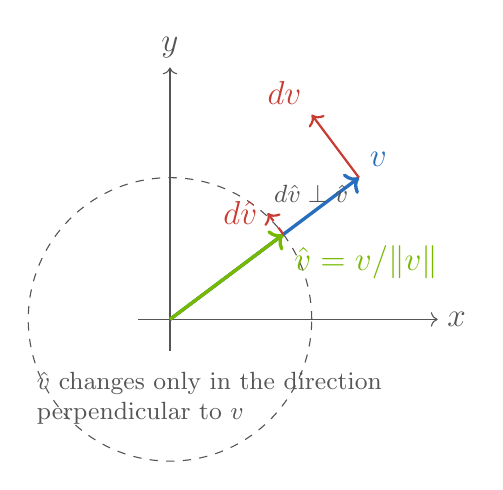
\begin{tikzpicture}[font=\large]
  % Left: geometry. Unit circle, vector v, unit vector vhat, tangent direction for dvhat.
  \coordinate (O) at (0,0);
  \draw[->, secG] (-0.4,0) -- (3.4,0) node[right] {$x$};
  \draw[->, secG] (0,-0.4) -- (0,3.2) node[above] {$y$};
  \draw[dashed, secG] (O) circle (1.8);
  % v = (2.4, 1.8), |v| = 3
  \draw[->, very thick, gsBlue] (O) -- (2.4,1.8) node[above right] {$v$};
  % vhat = v/|v| scaled to the unit circle
  \draw[->, very thick, cudaG] (O) -- (1.44,1.08) node[below right] {$\hat v=v/\lVert v\rVert$};
  % perturbation dv and its effect on vhat (tangential component only)
  \draw[->, thick, sadRed] (2.4,1.8) -- (2.4-0.6,1.8+0.8) node[above left] {$dv$};
  \draw[->, thick, dashed, sadRed] (1.44,1.08) -- (1.44-0.2,1.08+0.27) node[left] {$d\hat v$};
  \draw[secG] (1.2,1.6) node[right] {\small $d\hat v \perp \hat v$};
  \node[font=\small, secG, align=left] at (0.5,-1.0)
     {$\hat v$ changes only in the direction\\ perpendicular to $v$};
\end{tikzpicture}
\end{document}
